% !TEX root = ../../../main.tex
% 来源：中学数学实验教材·第三册（高中数学）
% 章节：二次函数 / 二次函数
% 原始文件：5.tex，行 781-796
% 类型：tikz
% ---
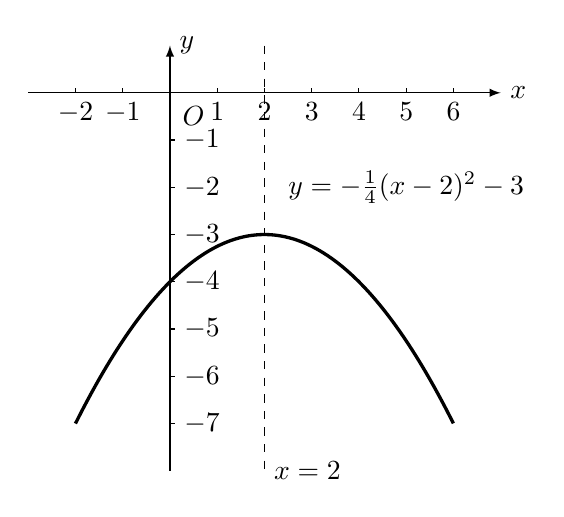
\begin{tikzpicture}[>=latex, scale=.6]
\draw[->] (-3,0)--(7,0)node[right]{$x$};
\draw[->] (0,-8)--(0,1)node[right]{$y$};
\foreach \x in {-2,-1,1,2,...,6}
{
    \draw (\x,0)node[below]{$\x$}--(\x,.1);
}
\foreach \y in {-1,-2,...,-7}
{
    \draw (0,\y)--(.1,\y)node[right]{$\y$};
}
\node at (.5,-.5){$O$};
\draw [domain=-2:6, samples=100, very thick]plot(\x, {-.25*(\x-2)*(\x-2)-3});
\draw[dashed](2,1)--(2,-8)node[right]{$x=2$};
\node at (5,-2){$y=-\frac{1}{4}(x-2)^2-3$};
\end{tikzpicture}
